\documentclass[a4paper,11pt]{article}
\usepackage[utf8]{inputenc}
\usepackage[T1]{fontenc}
\renewcommand{\figurename}{Obrázok}
\usepackage{graphicx}
\usepackage[margin=2cm]{geometry}
\usepackage{float}

\begin{document}
\section*{Simulácia PMOS ochrany napájania}

\begin{figure}[H]
  \centering
  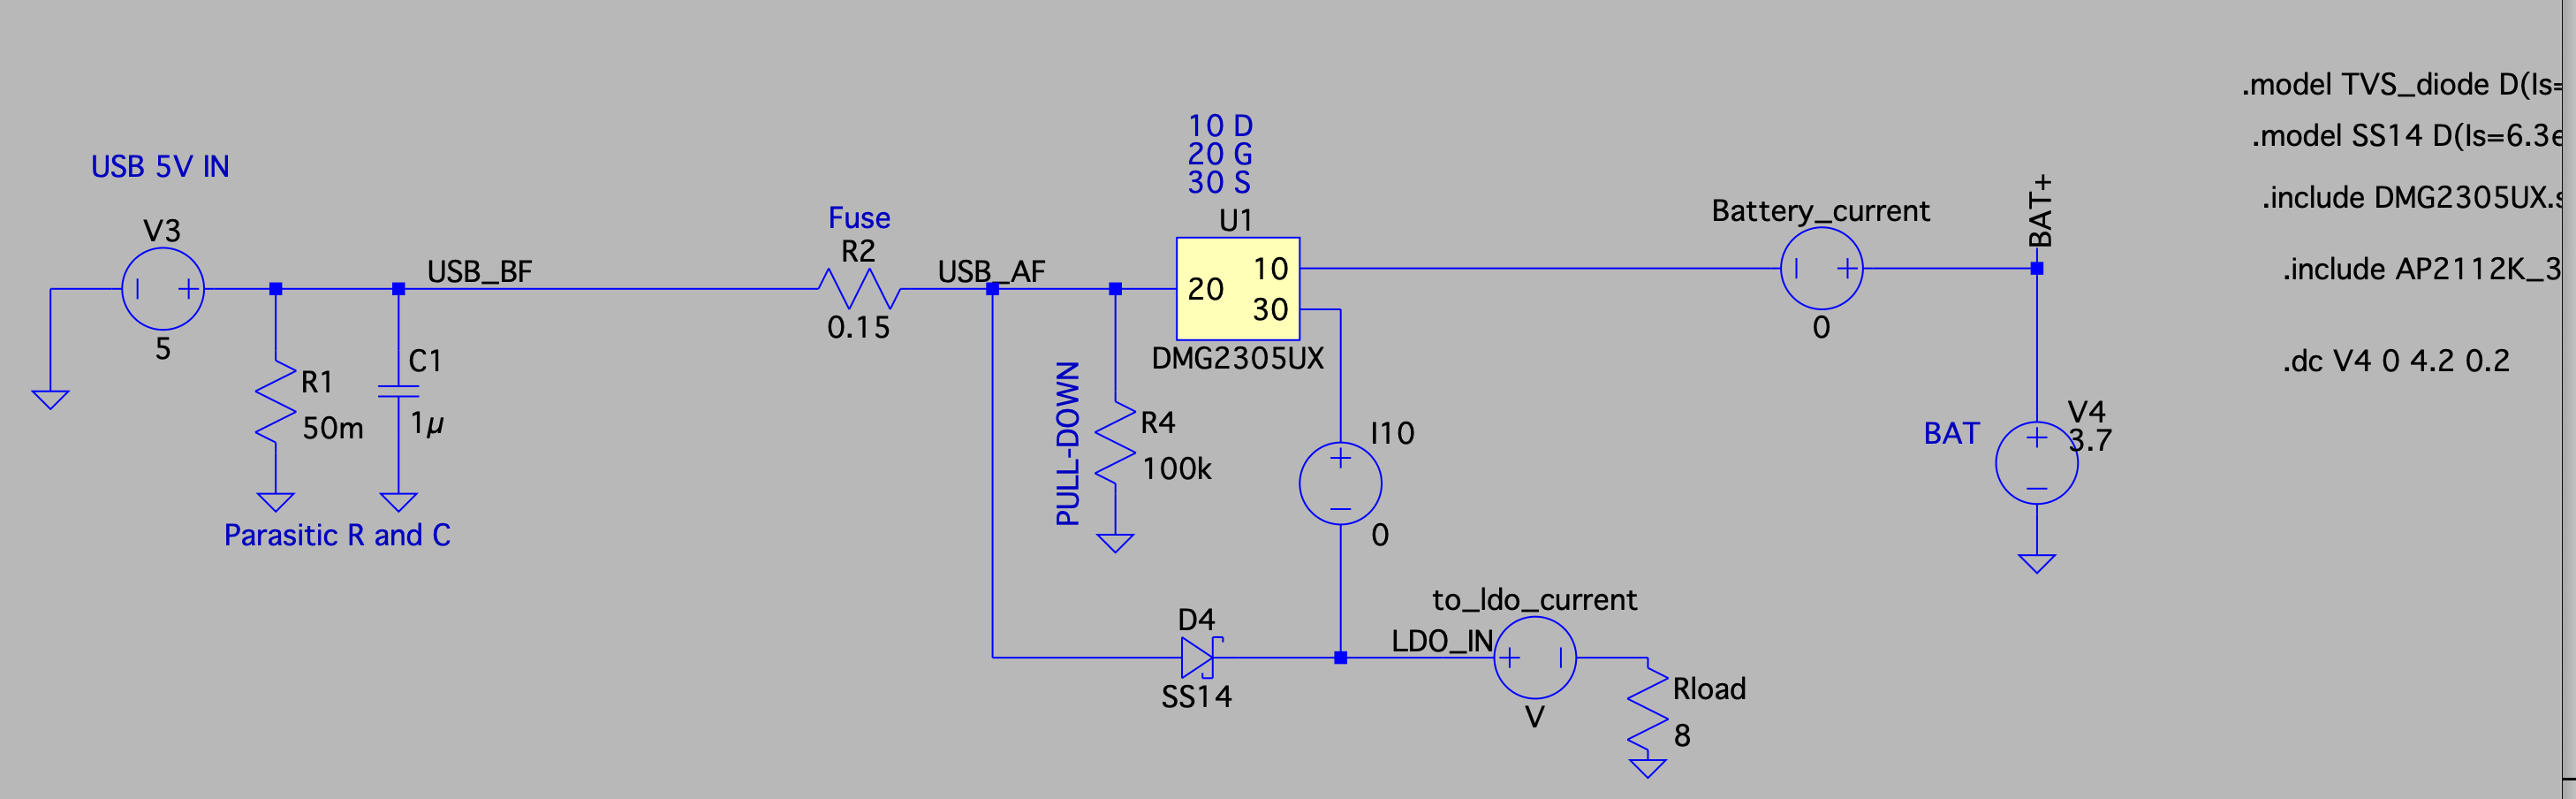
\includegraphics[width=\textwidth]{schema.png}
  \caption{Simulačná schéma}
\end{figure}

V3 sa meni medzi 5V a 0V.

\subsection*{USB = 5\,V -- prúd unikajúci do batérie}

\begin{figure}[H]
  \centering
  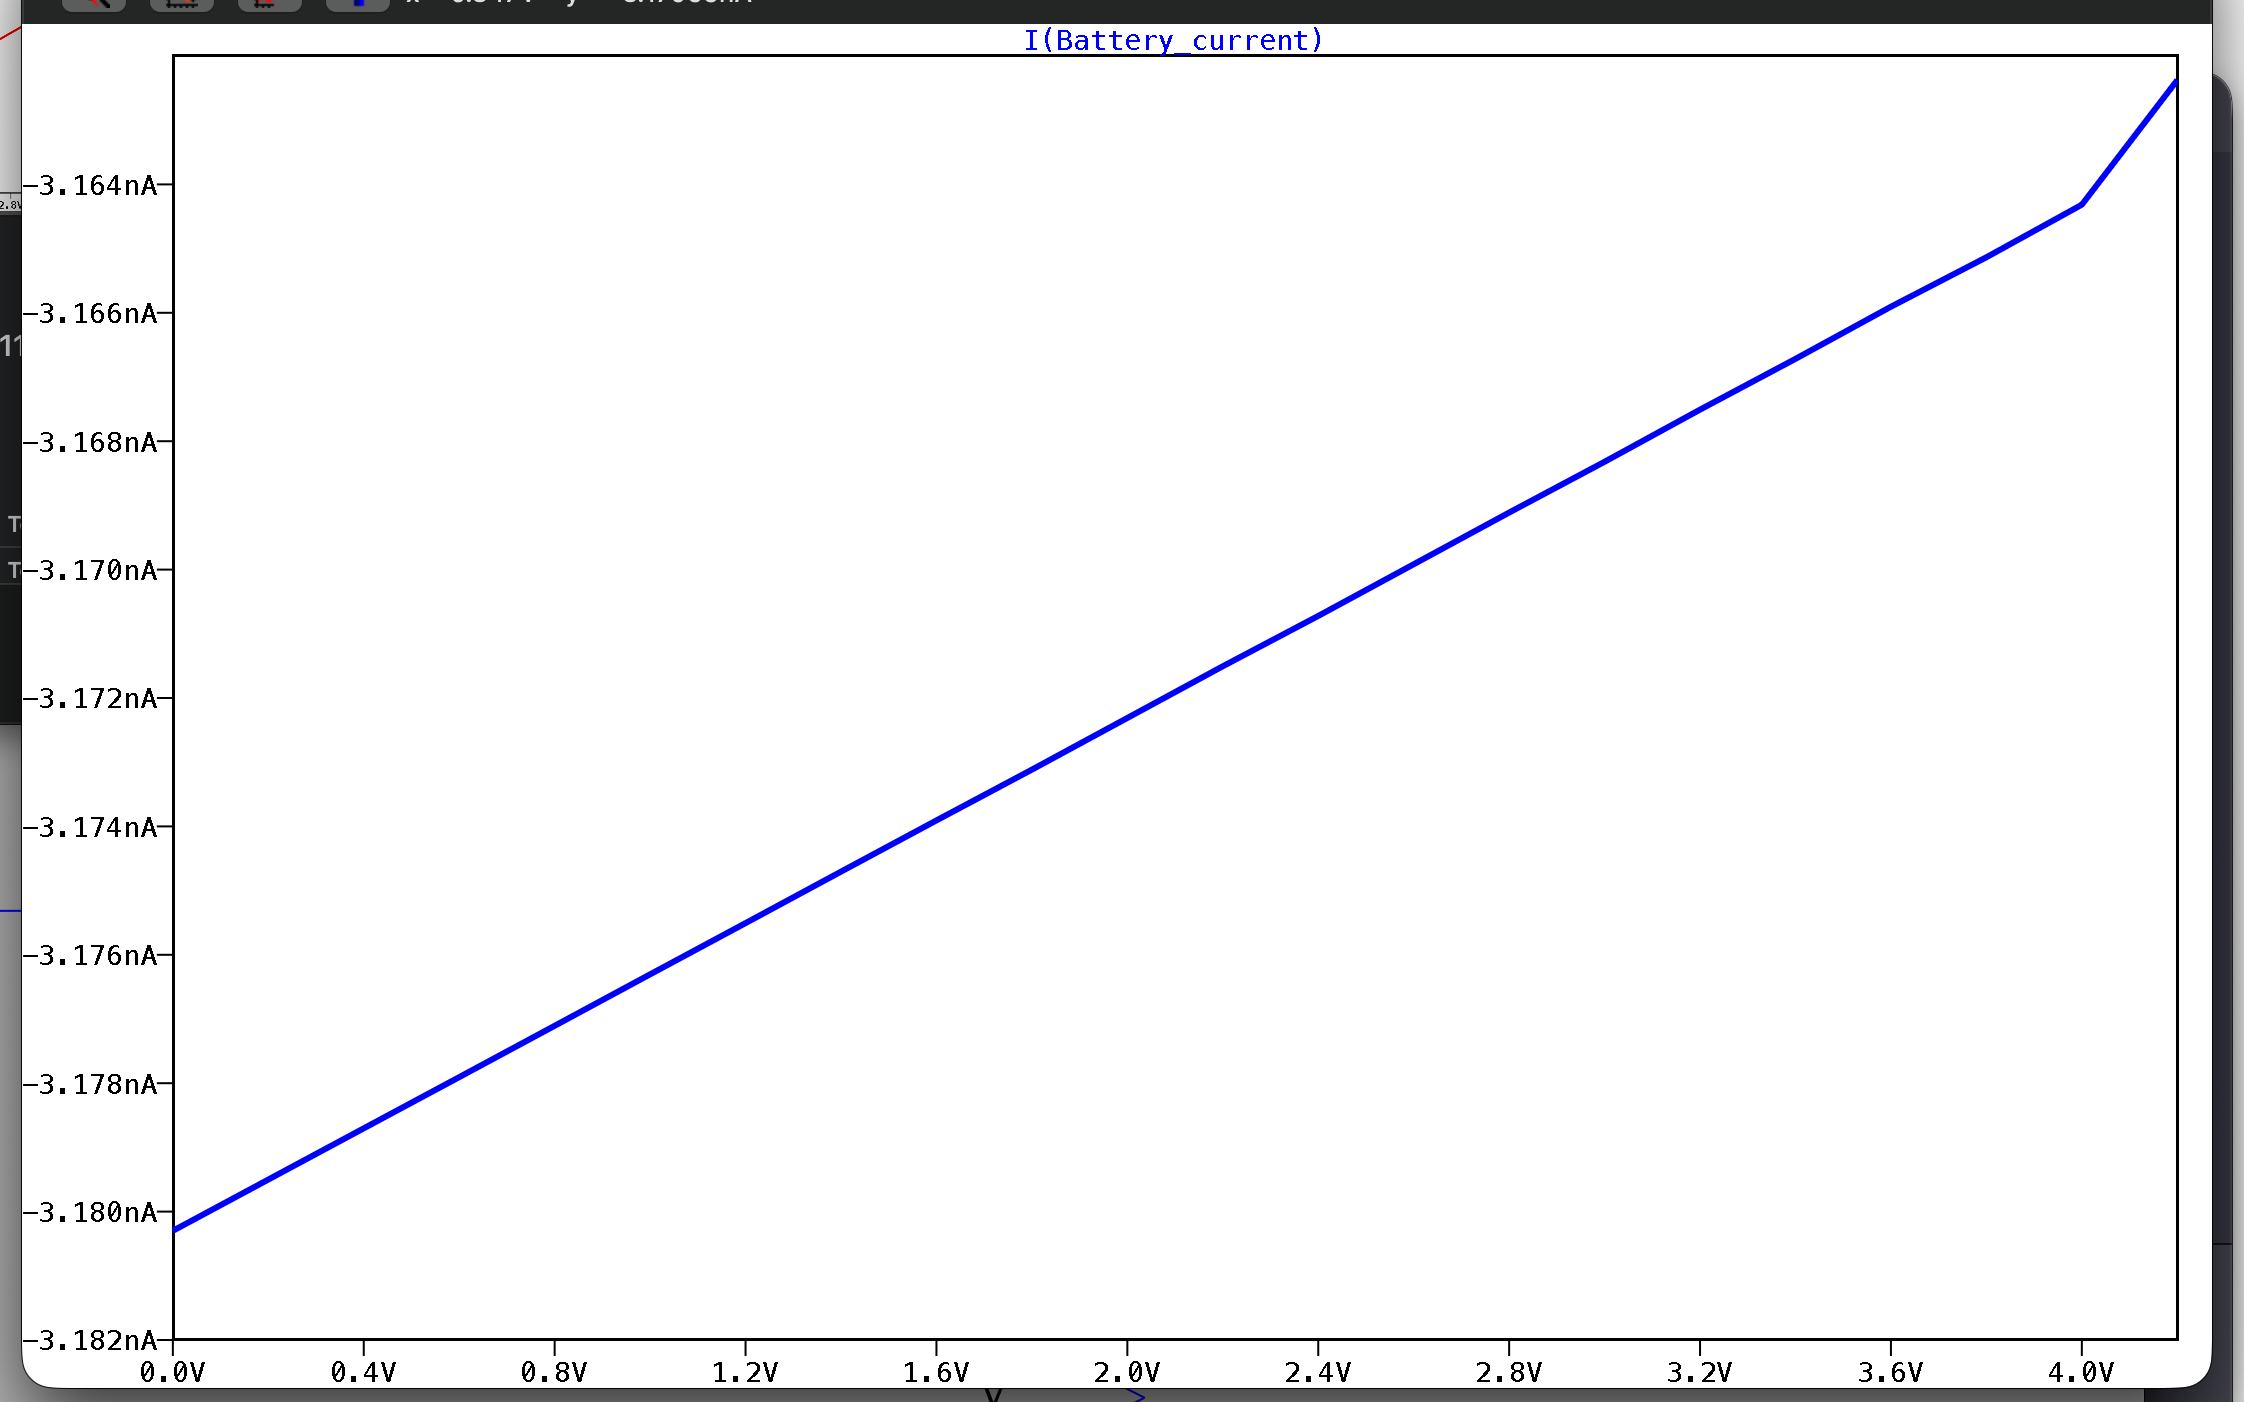
\includegraphics[width=0.85\textwidth]{leakage_pmos_5v.png}
  \caption{Prúd do batérie}
\end{figure}

Leakage okolo 3nA. V najhoršom prípade je rozdiel medzi S-D 2V ktoré by body dioda mala vydržať.

\begin{figure}[H]
  \centering
  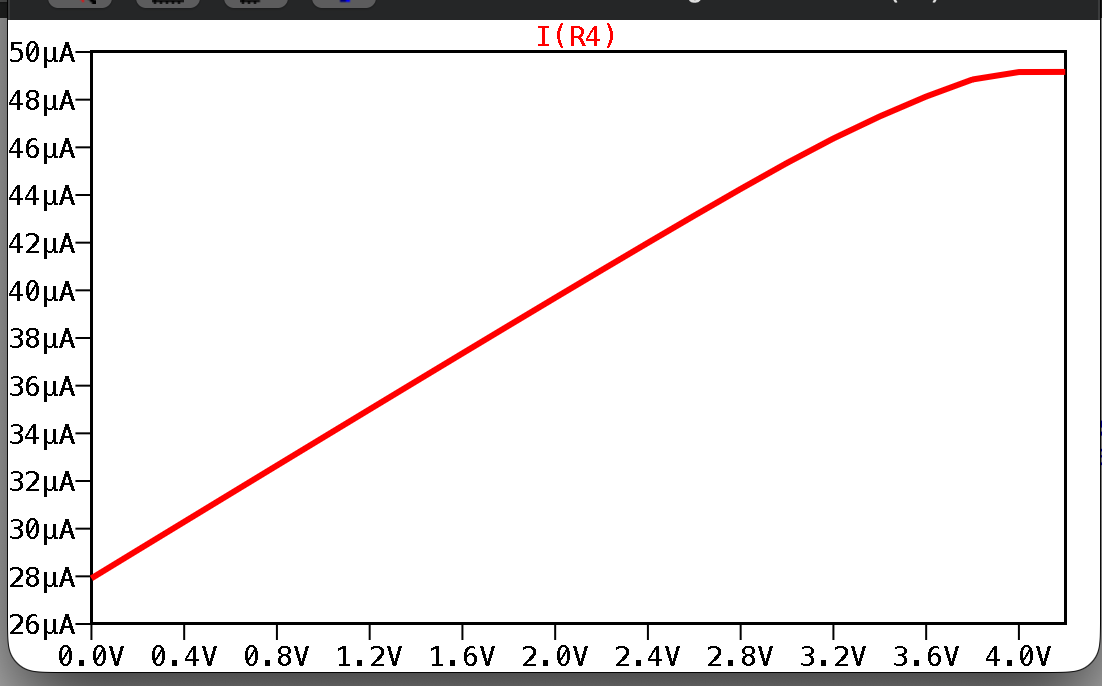
\includegraphics[width=0.85\textwidth]{prud_pull_down.png}
  \caption{Prúd pull-down rezistorom $I(R4)$ pri USB = 5\,}
\end{figure}

50uA znie fajn

\subsection*{USB = 0\,V -- normálna prevádzka z batérie}

\begin{figure}[H]
  \centering
  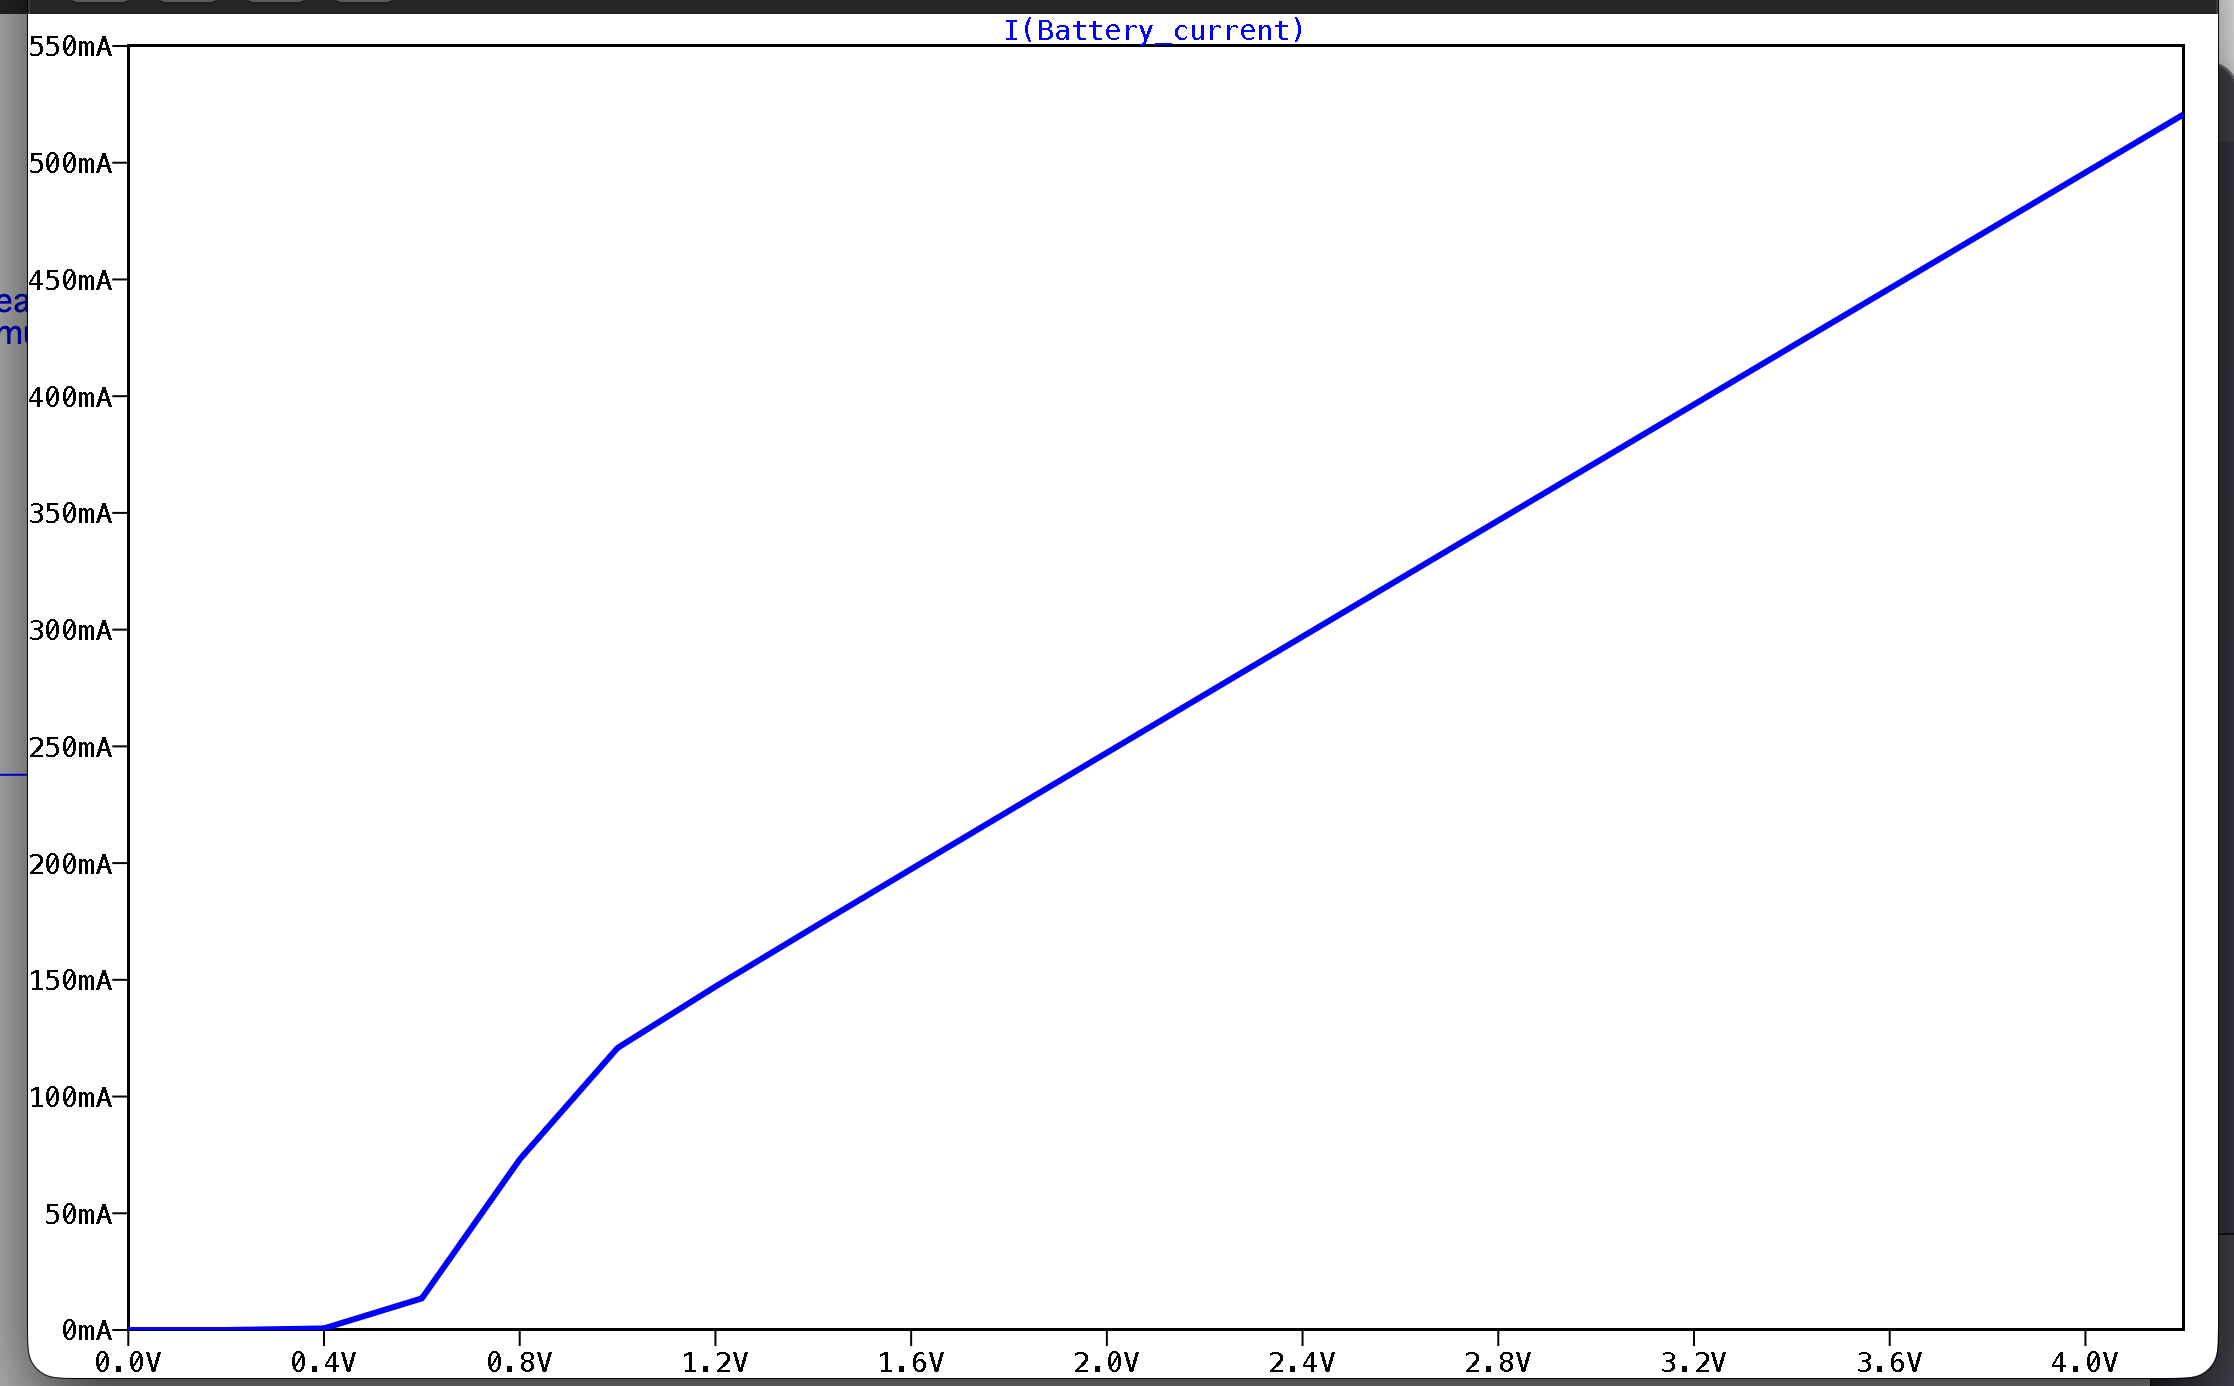
\includegraphics[width=0.85\textwidth]{battery_current_0v.png}
  \caption{Prúd odoberaný z batérie pri USB = 0\,V}
\end{figure}

\begin{figure}[H]
  \centering
  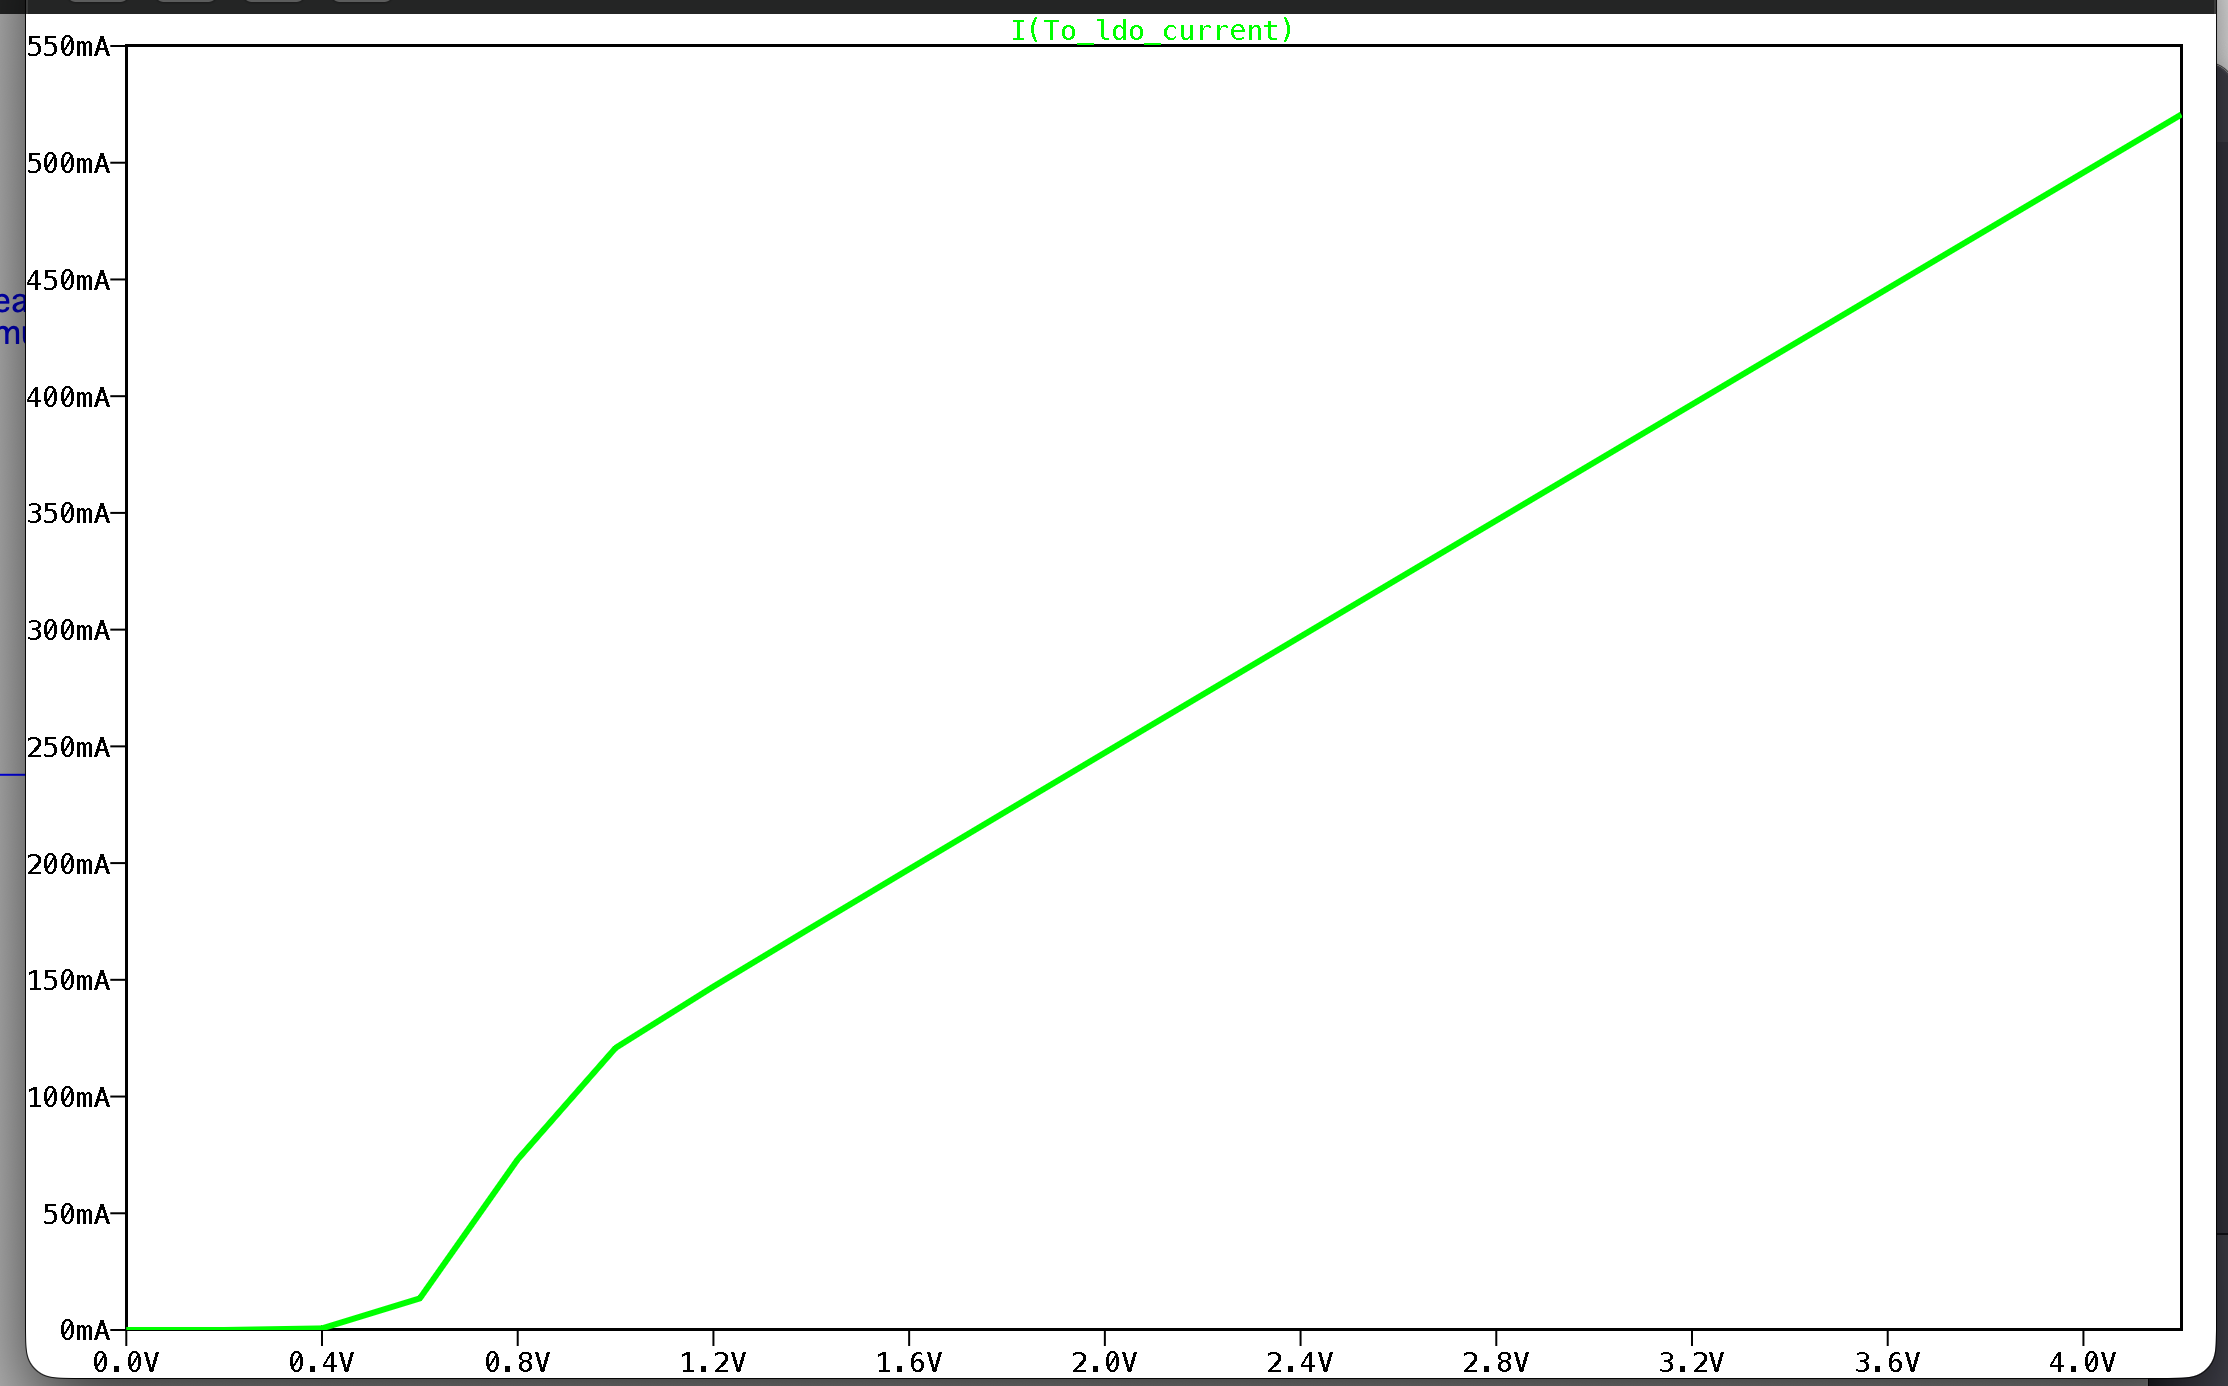
\includegraphics[width=0.85\textwidth]{current_to_ldo_0V.png}
  \caption{Prúd do LDO pri USB = 0\,V}
\end{figure}

 Zhoduje sa s prúdom batérie, takže všetok prúd prechádza cez PMOS.

\subsection*{Nová navrhovaná schéma}

\begin{figure}[H]
  \centering
  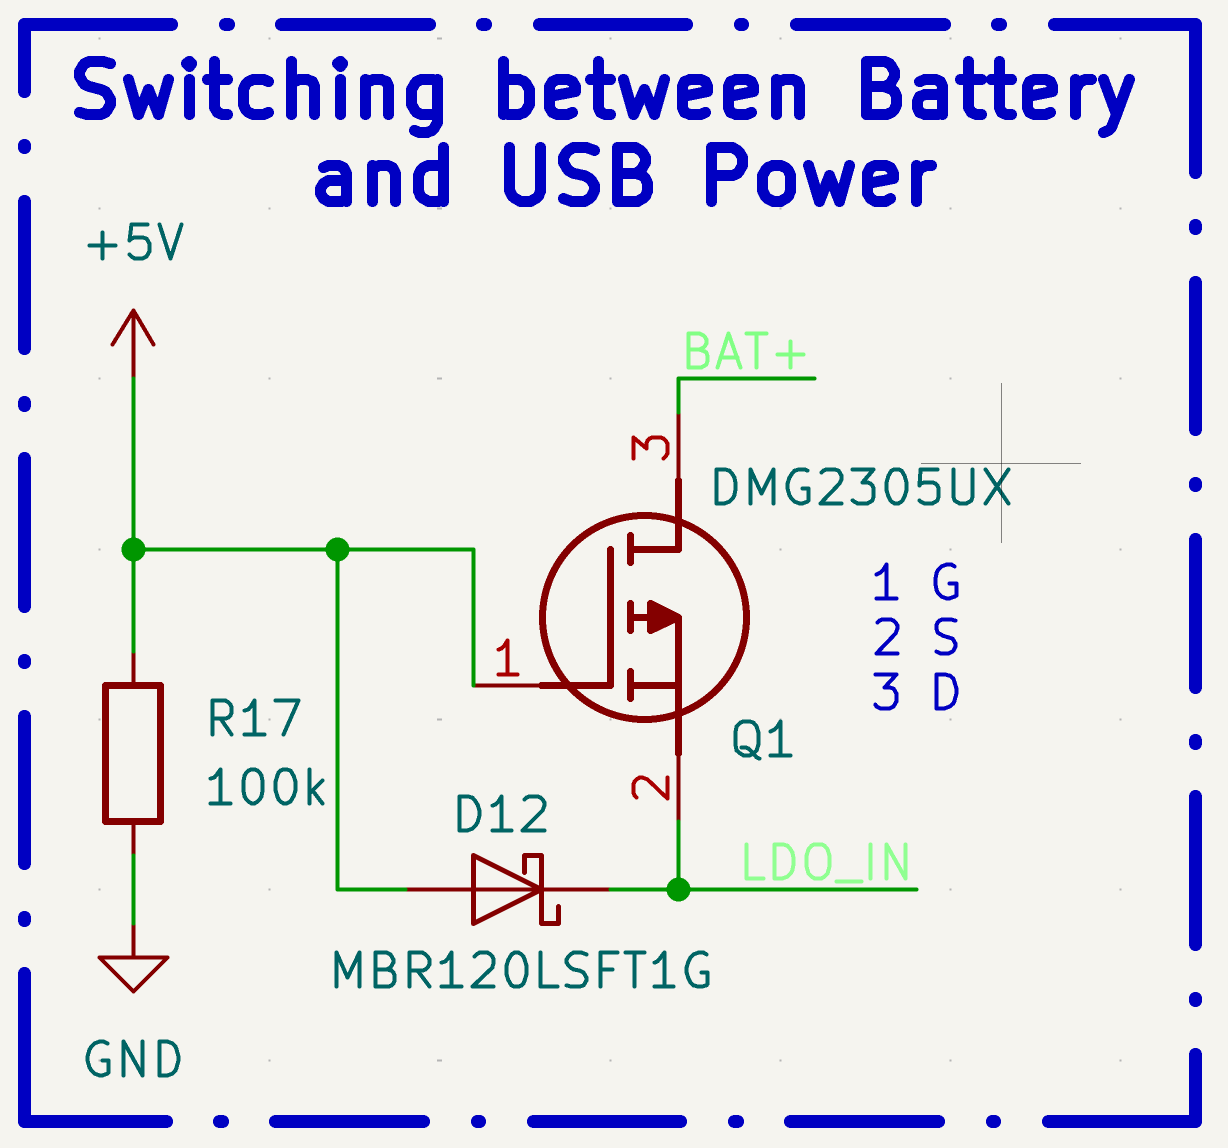
\includegraphics[width=0.6\textwidth]{new_board_connection.png}
  \caption{Nové zapojenie PMOS (Q1)}
\end{figure}
\end{document}
